\chapter{Multi-Sensor Array}
The ML analysis was recorded for three sensors, and each sensor was maintained at a sufficiently high temperature in order to achieve a decent sensor response. However, each sensor material (oxides in this case) may have its optimum temperature at which the response would be highest, and this optimum response temperature need not be the same for all materials used. Therefore, compared to the previous method of measurement, where all the sensors are kept at the same temperature (See Appendix C), a new setup was designed and built wherein a sizable number of sensor arrays (6 nodes) may be accommodated. The temperature of each can be controlled individually such that each of them is at its optimal temperature. Besides, one can also program the heater power supply to the desired waveform to tune the sensor response dynamically, and that could be used as an effective control feature of ML data.
\begin{figure}
    \centering
    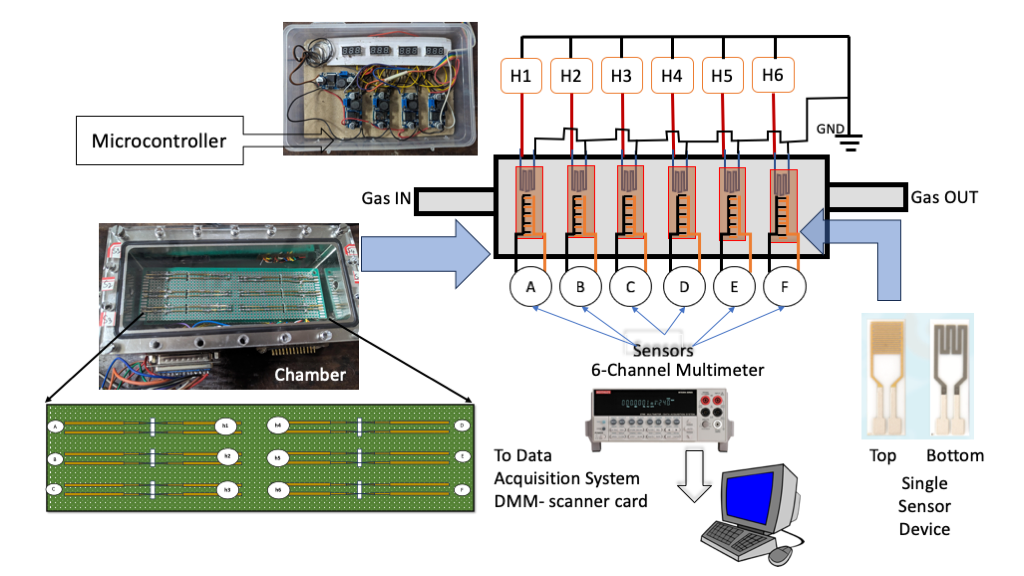
\includegraphics[width=1\linewidth]{Thesis Prashant//Images//Figures/Picture_presentation.png}
    \caption{Schematics of six sensor arrays with individual heater control using microcontroller and the sensor output leads (Interdigitated gold electrodes) to simultaneously measure sensor response of 6 nodes. The typical single-sensor device is shown with top electrodes and a bottom heater.}
    \label{setupl}
\end{figure}

The new setup built is shown in Fig 5.1. It can accommodate up to six sensors simultaneously, as seen in the figure. A metallic chamber containing two layers where one PCB Snaps on the other and holds the top PCB consist of six-hole slits where alumina samples with deposited heaters can be slid. On each side horizontal to the PCB slit, two pogo pins were used to make contact with the alumina sample electrode or heater, exploiting the spring-loaded mechanism of pogo pins. Similarly, six samples may be fitted in a single top PCB. The other side of the PCB contains 2.54 mm pins, which simply snap onto the bottom PCB. The Bottom PCB is fixed inside the chamber with all the wiring and connection to a 25-pin connector side to the wall of the chamber, as shown in the figure. A transparent lid is used to enclose the chamber from the top. The metal chamber has inlet and outlet pipes to achieve gas flow. 

The whole assembly consist of six sensors and six heaters. The Pt deposition on the alumina substrate on one side acts as a heater with $6 \Omega$ resistance, ensuring precise and local heating. On the other hand, the opposite side of the alumina provides the surface for the sensor substrate. A multi-channel voltage supply was also constructed using a parallel six-buck converter to drive the heater at a constant temperature individually. The main voltage source for all the buck converters was a 24 V-5 A SMPS (Switch Mode Power Supply). The buck converter gives the freedom to adjust the constant voltage individually by changing its potentiometer. Hence temperature of the each sensor can be controlled, for better utilization a micro controller can be used to set the temperature simultaneously for each sensor by changing the voltage on buck converter. The heater can go up to $450^\circ C$ at 12 V. So the Bottom PCB inside the chamber provides the interface to connect all the sensors to the voltage supply source and multi-meter to measure the resistance. 

\begin{figure}
    \centering
    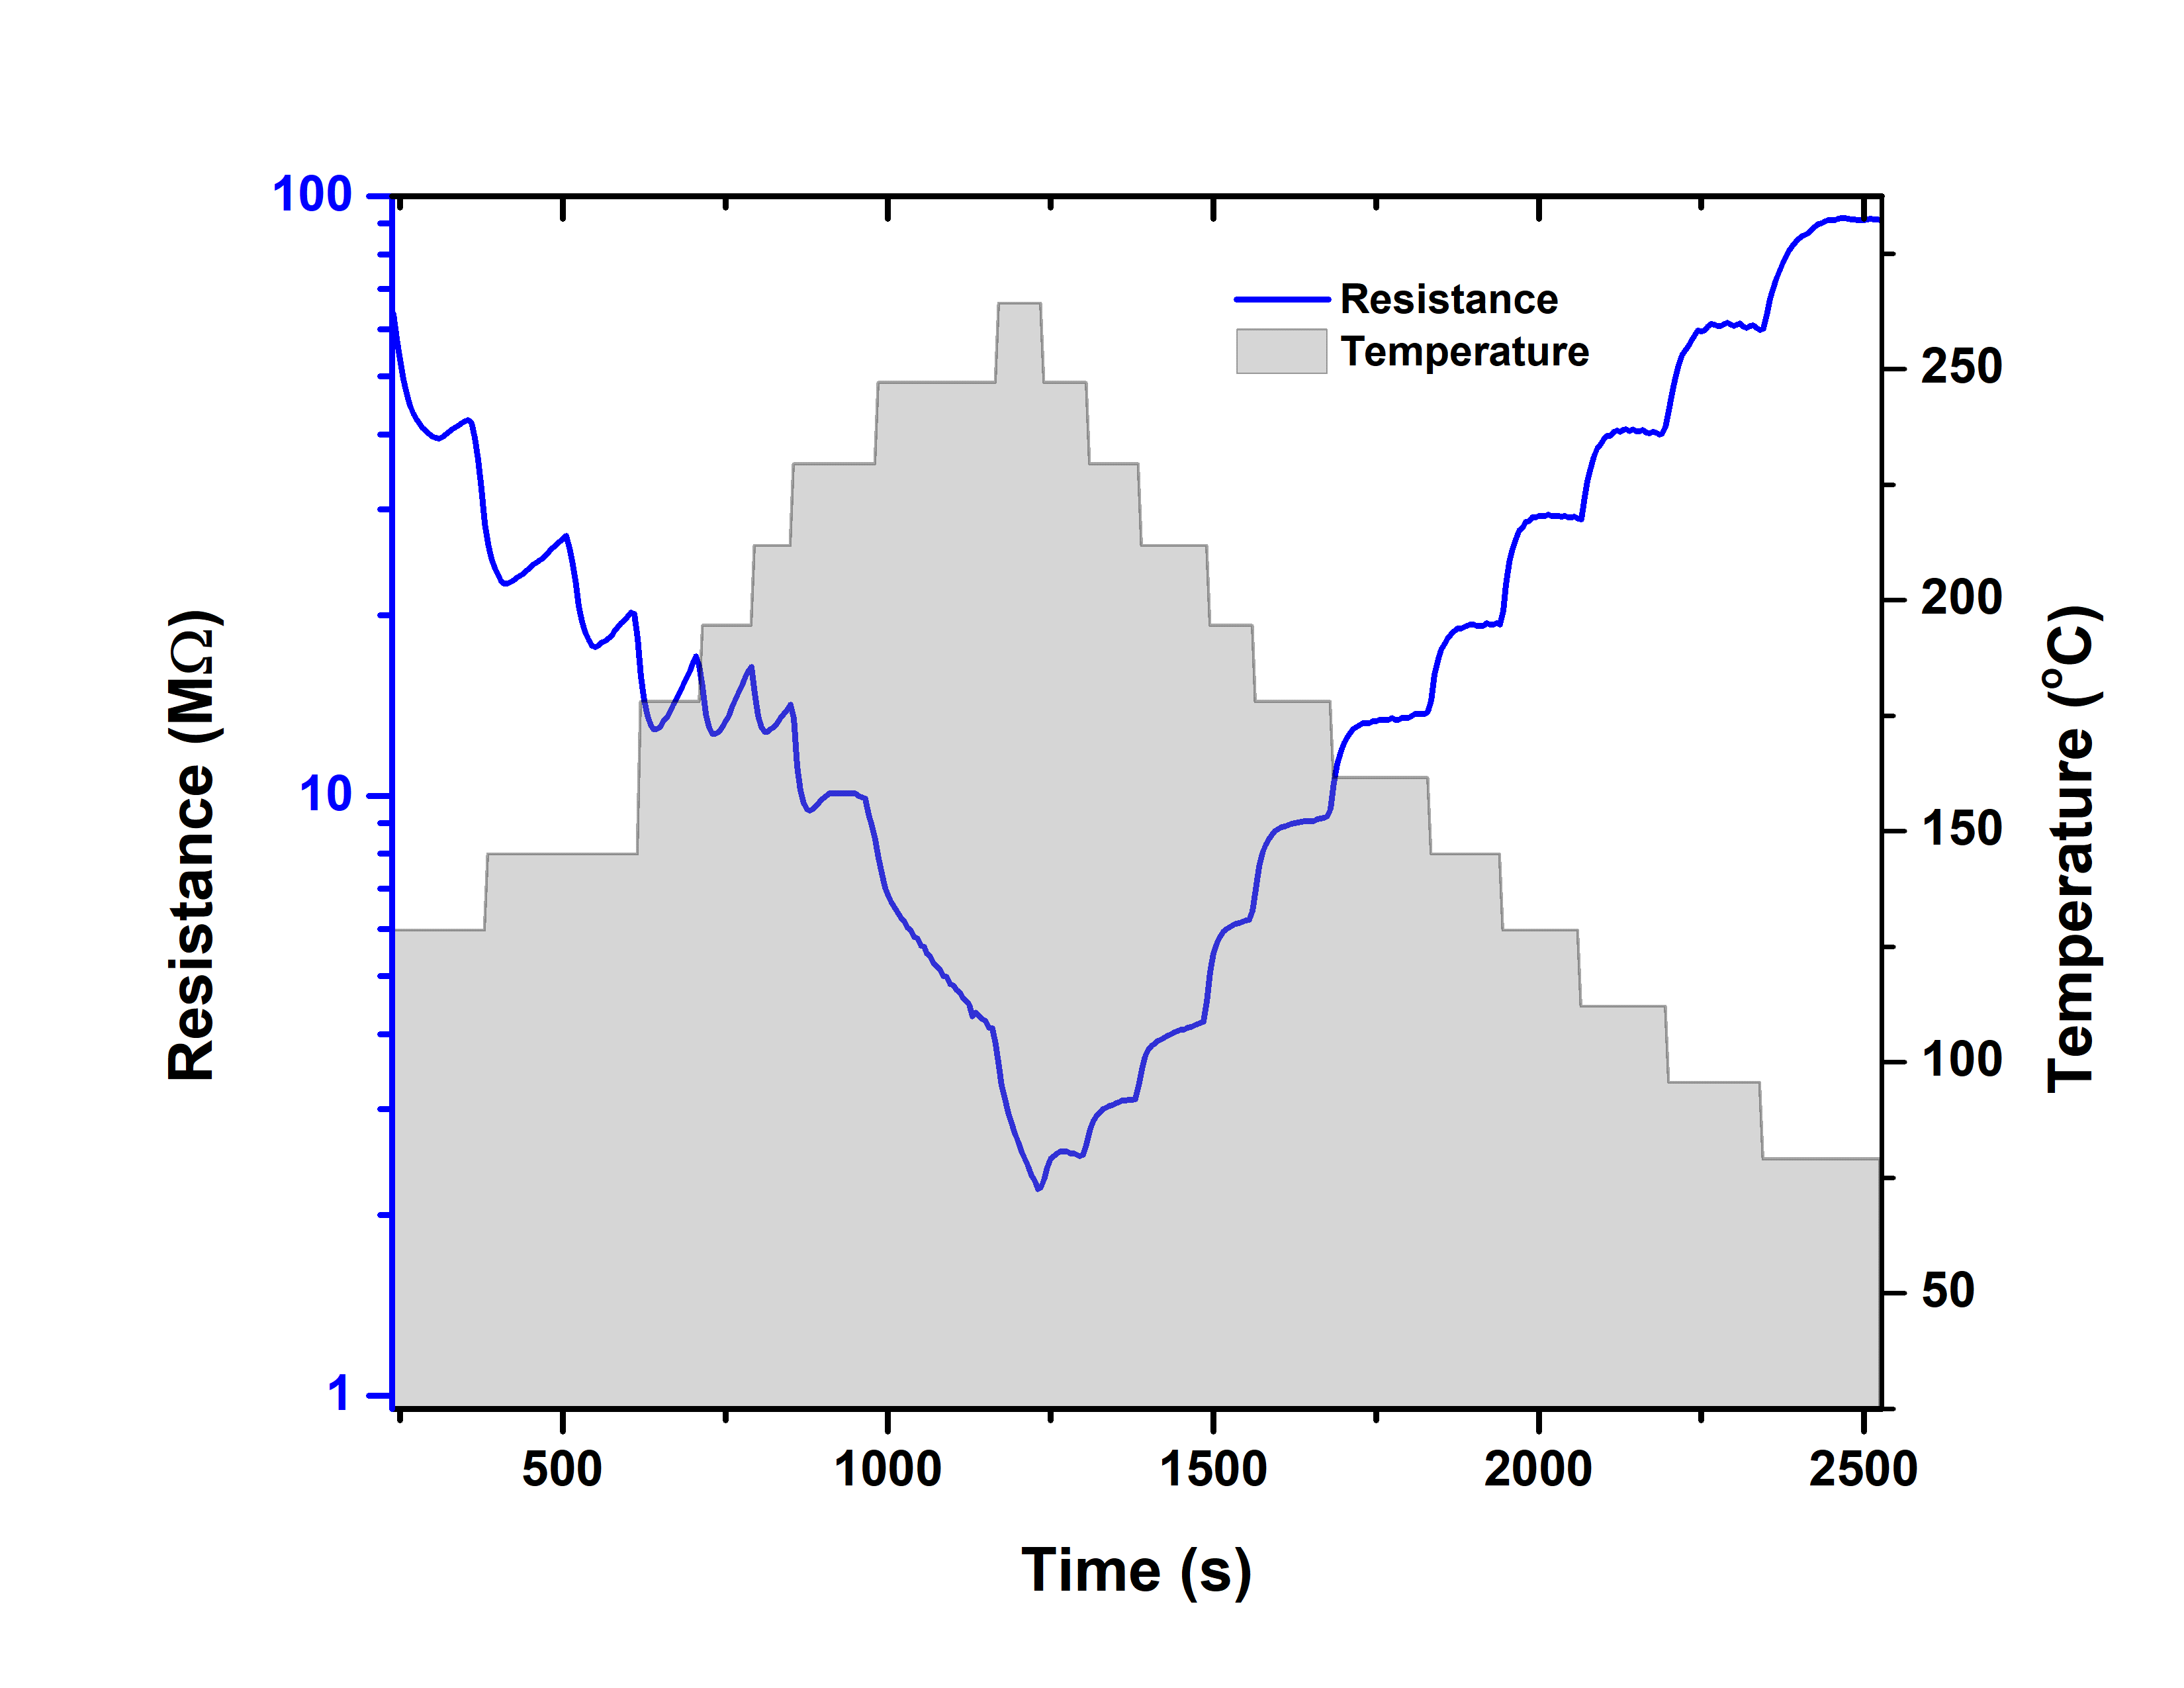
\includegraphics[width=1\linewidth]{Thesis Prashant//Images//Figures/Graph10.png}
    \caption{The data recorded with the assembly described in Fig 5.1 for a single sensor using a controller made. (measurement courtesy Ms. Niharika)}
    \label{fig:setup}
\end{figure}


